%%%%%%%%%%%%%%%%%%%%%%%%%%%%%%%%%%%%%%%%%%%%%%%%%%%%%%%%%%%%%%%%%%%%%%%%%%
%%
%%	Author Submission Template for Operations Research (OPRE)
%%	INFORMS, <informs@informs.org>
%%	Ver. 1.00, June 2024
%%  Modified by Jiheng Zhang @ UST
%%
%%%%%%%%%%%%%%%%%%%%%%%%%%%%%%%%%%%%%%%%%%%%%%%%%%%%%%%%%%%%%%%%%%%%%%%%%%
%
% Use dblanonrev for Double Anonymous Review submission
% Use sglanonrev for Single Anonymous Review submission
% For example, submission to INFORMS Mathematics of Operation Research, MOOR will have
% \documentclass[moor,dblanonrev]{informs4}
%
% \documentclass[opre,dblanonrev]{informs4}
\documentclass[opre,sglanonrev]{informs4}
% \usepackage{eqndefns-left} % For checking the display equation width and equation environment definitions %
\RequirePackage{tgtermes}
\RequirePackage{newtxtext}
\RequirePackage{newtxmath}
\RequirePackage{bm}
\RequirePackage{endnotes}

% Load the fix-cm package
\usepackage{fix-cm}
% Manually declare missing font shapes if necessary
\DeclareFontShape{OML}{cmm}{b}{it}{<->cmmib10}{}
\DeclareFontShape{OMS}{cmsy}{b}{n}{<->cmsy10}{}

%\OneAndAHalfSpacedXI
\OneAndAHalfSpacedXII % Current default line spacing
%%\DoubleSpacedXI
%%\DoubleSpacedXII

% Optional LaTeX Packages
\usepackage{algorithm}
\usepackage{algpseudocode}
\usepackage{tikz}
% Private macros here (check that there is no clash with the style)

\usepackage{hyperref}       % hyperlinks
\hypersetup{
  colorlinks=true,
  linkcolor=red,
  urlcolor=magenta,
  citecolor=blue
}

% Natbib setup for author-number style
\usepackage{natbib}
 \bibpunct[, ]{(}{)}{,}{a}{}{,}%
 \def\bibfont{\small}%
 \def\bibsep{\smallskipamount}%
 \def\bibhang{24pt}%
 \def\newblock{\ }%
 \def\BIBand{and}%


%% Setup of the equation numbering system. Outcomment only one.
%% Preferred default is the first option.
\EquationsNumberedThrough    % Default: (1), (2), ...
%\EquationsNumberedBySection % (1.1), (1.2), ...

%% Setup of theorem styles. Outcomment only one.
%% Preferred default is the first option.
\TheoremsNumberedThrough     % Preferred (Theorem 1, Lemma 1, Theorem 2)
%\TheoremsNumberedByChapter  % (Theorem 1.1, Lema 1.1, Theorem 1.2)
\ECRepeatTheorems  %  

% For new submissions, leave this number blank.
% For revisions, input the manuscript number assigned by the on-line
% system along with a suffix ".Rx" where x is the revision number.
\MANUSCRIPTNO{MOOR-0001-2024.00}

%%%%%%%%%%%%%%%%
\begin{document}
%%%%%%%%%%%%%%%%

% Outcomment only when entries are known. Otherwise leave as is and
%   default values will be used.
%\setcounter{page}{1}
%\VOLUME{00}%
%\NO{0}%
%\MONTH{Xxxxx}% (month or a similar seasonal id)
%\YEAR{0000}% e.g., 2005
%\FIRSTPAGE{000}%
%\LASTPAGE{000}%
%\SHORTYEAR{00}% shortened year (two-digit)
%\ISSUE{0000} %
%\LONGFIRSTPAGE{0001} %
%\DOI{10.1287/xxxx.0000.0000}%

% Author's names for the running heads
% Sample depending on the number of authors;
% \RUNAUTHOR{Jones}
% \RUNAUTHOR{Jones and Wilson}
% \RUNAUTHOR{Jones, Miller, and Wilson}
% \RUNAUTHOR{Jones et al.} % for four or more authors
% Enter authors following the given pattern:
%\RUNAUTHOR{}

% Title or shortened title suitable for running heads. Sample:
% \RUNTITLE{}


% Enter the full title:
\TITLE{Optimal Resource Allocation in Humanitarian Logistics: A Stochastic Programming Approach}

% Block of authors and their affiliations starts here:
% NOTE: Authors with same affiliation, if the order of authors allows,
%   should be entered in ONE field, separated by a comma.
%   \EMAIL field can be repeated if more than one author
\ARTICLEAUTHORS{%
%\AUTHOR{John Doe,\textsuperscript{a} Jane Smith,\textsuperscript{b}}
%\AFF{\textsuperscript{a}Department of Industrial Engineering, University of XYZ, \EMAIL{john.doe@xyz.edu; \textsuperscript{b}Department of Computer Science, University of ABC, \EMAIL{jane.smith@abc.edu}} 
\AUTHOR{John Smith}
\AFF{Department of Logistics,
University of XYZ, \EMAIL{john.smith@xyz.edu}}

\AUTHOR{Emily Johnson}
\AFF{Department of Logistics,
University of ABC, \EMAIL{emily.johnson@abc.edu}}
% Enter all authors
} % end of the block

\ABSTRACT{%
% Enter your abstract
In humanitarian logistics, efficient resource allocation is paramount for ensuring timely and effective delivery of aid to populations in need. This paper presents a novel approach to optimize resource allocation in humanitarian logistics using stochastic programming. By integrating stochastic elements into the modeling framework, our approach accounts for uncertainty in demand, supply, and transportation constraints, providing decision-makers with robust and adaptable solutions. We develop a mixed-integer linear programming formulation to minimize the total cost of relief operations while meeting demand requirements under varying scenarios. Through computational experiments and a case study, we demonstrate the effectiveness of our approach in improving decision-making and resource utilization in humanitarian relief efforts. Our findings underscore the importance of incorporating stochastic programming techniques in addressing the complex challenges of humanitarian logistics.
}%

%\FUNDING{This research was supported by [grant number, funding agency].}

\KEYWORDS{Stochastic programming, Decision support,Uncertainty, Disaster response, Optimization} 

%\HISTORY{Received: Month DD, YYYY; Accepted: Month DD, YYYY; Published Online: Month DD, YYYY}

\maketitle
%%%%%%%%%%%%%%%%%%%%%%%%%%%%%%%%%%%%%%%%%%%%%%%%%%%%%%%%%%%%%%%%%%%%%%

% Text of your paper here

\section{Introduction}\label{sec:Intro}

Humanitarian crises, such as natural disasters, conflicts, and pandemics, often result in widespread devastation, displacing populations and disrupting essential services. Timely and effective delivery of humanitarian aid is crucial to mitigate the impact of such crises and save lives~\cite{smith2005}. However, humanitarian logistics operations face numerous challenges, including uncertainty in demand, limited resources, logistical constraints, and dynamic operating environments. Optimal resource allocation plays a central role in addressing these challenges by ensuring that available resources are allocated efficiently to meet the needs of affected populations.
\begin{equation}
\mathrm{Cost\_Red}_j=\rho_0+\rho_1N_{m_j}
+\rho_2N_{l_j}+\rho_3I2_{m_j}+\rho_4I2_{l_j}
+\rho_5OS_{m_j}+\phi\mathbf{X}_j+\mu_j
\end{equation}

In recent years, there has been growing interest in applying mathematical optimization techniques to improve the efficiency and effectiveness of humanitarian logistics operations. Traditional approaches typically rely on deterministic models that assume perfect information and static conditions. However, in practice, humanitarian crises are characterized by uncertainty and variability, making it essential to incorporate stochastic elements into the modeling process. Stochastic programming offers a powerful framework for addressing uncertainty and optimizing decision-making under uncertain conditions.
\begin{align}
\mbox{Cost\_Red}_j&=\rho_0+\rho_1N_{m_j}+\rho_2N_{l_j}+\rho_3I2_{m_j}\notag\\
&\quad+\rho_4I2_{l_j}+\rho_5OS_{m_j}+\phi\mathbf{X}_j+\mu_j
\end{align}

In this paper, we present a stochastic programming approach to optimize resource allocation in humanitarian logistics~\citep{jones2010}. Our approach aims to balance the trade-off between cost minimization and service quality while considering uncertainty in demand, supply, and transportation constraints. We develop a mixed-integer linear programming (MILP) formulation that captures the stochastic nature of humanitarian crises and provides decision support for relief agencies. The proposed model integrates both deterministic and stochastic components, allowing decision-makers to make informed decisions in uncertain environments.

\section{Methodology}\label{sec:Method}
We formulate the resource allocation problem as a two-stage stochastic programming problem, where the first stage involves decisions on resource allocation and the second stage represents the realization of uncertain parameters~\citep{smith2005,jones2010,brown2015}. The objective is to minimize the total cost of relief operations, including procurement, transportation, and distribution costs, subject to various constraints, such as capacity constraints, demand satisfaction requirements, and budget constraints.

The cost function $C(x)$ is defined as the sum of procurement, transportation, and distribution costs:
\begin{equation}
C(x) = \sum_{i=1}^{n} \Biggl(c_i p_i + \sum_{j=1}^{m} d_{ij} t_{ij} + \sum_{k=1}^{l} s_k q_k\Biggr)
\end{equation}

We model uncertainty using scenario-based stochastic programming, where multiple scenarios representing different realizations of uncertain parameters are considered. We use historical data, expert opinions, and probabilistic forecasts to generate scenario sets that capture the range of possible outcomes. The stochastic programming model then generates optimal resource allocation decisions that minimize the expected total cost across all scenarios while ensuring robustness against uncertainty.

The objective function of the stochastic programming model is formulated as follows:
\begin{equation*}
\min_{x,y} \quad \sum_{s \in S} \left[ f(x, y, s) \cdot \mathbb{P}(s) \right]
\end{equation*}
subject to:
\begin{align}
g(x, y, s) \leq 0 &\quad \forall s \in S\\
h(x, y, s) = 0 &\quad \forall s \in S
\end{align}

\begin{theorem}[Optimality Conditions]\label{thm:Opt}
Let $x^*$ be an optimal solution to the stochastic programming problem. If the objective function and constraint functions are convex, then $x^*$ satisfies the Karush-Kuhn-Tucker (KKT) conditions.
\end{theorem}

\begin{proof}{Proof}
The proof follows from the convex optimization theory, which states that for convex objective and constraint functions, the KKT conditions are necessary and sufficient for optimality. Therefore, if $x^*$ is an optimal solution, it must satisfy the KKT conditions.\Halmos
\end{proof}

\begin{algorithm}
\caption{Random Forest Training}
\vskip6pt
\begin{algorithmic}
\Procedure{RandomForest}{$X_{\text{train}}, y_{\text{train}}, \text{num\_trees}$}
    \State forest $\gets []$
    \For{$i \gets 1$ \textbf{to} $\text{num\_trees}$}
        \State $X_{\text{sampled}}, y_{\text{sampled}} \gets \text{bootstrap\_sample}(X_{\text{train}}, y_{\text{train}})$
        \State tree $\gets$ \Call{DecisionTree}{$X_{\text{sampled}}, y_{\text{sampled}}$}
        \State \textbf{append} tree to forest
    \EndFor
    \State \textbf{return} forest
\EndProcedure
\Statex
\end{algorithmic}
\end{algorithm}

 \begin{figure}
     \FIGURE
 %    {\includegraphics{figure-filename.pdf}} %Callout External Image
 %	Include LaTeX figures
 {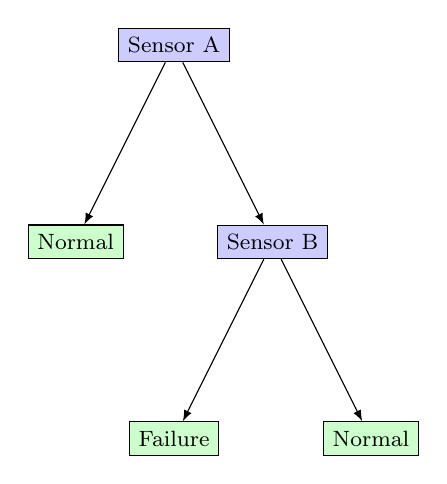
\begin{tikzpicture}[
  grow=down,
  level 1/.style={sibling distance=2.5cm, level distance=2.5cm},
  edge from parent/.style={draw,-latex},
  every node/.style={font=\footnotesize},
  decision/.style={shape=rectangle,draw,fill=blue!20},
  leaf/.style={shape=rectangle,draw,fill=green!20}
]
\node [decision] {Sensor A}
  child { node [leaf] {Normal} }
  child { node [decision] {Sensor B}
    child { node [leaf] {Failure} }
    child { node [leaf] {Normal} }
  };
\end{tikzpicture}}
{Text of the Figure Caption. \label{fig1}}
{Text of the notes.}
\end{figure}

\begin{algorithm}
\begin{algorithmic}[1]
\caption{Random Forest Training II}
\Procedure{DecisionTree}{$X, y$}
    \If{\textsc{StoppingCondition}$(X, y)$}
        \State \textbf{return} LeafNode$(y)$
    \Else
        \State $(\text{feature}, \text{threshold}) \gets \textsc{FindBestSplit}(X, y)$
        \State $\textit{left\_indices} \gets X[\text{feature}] \leq \text{threshold}$
        \State $\textit{right\_indices} \gets X[\text{feature}] > \text{threshold}$
        \State $\textit{left\_subtree} \gets$ \Call{DecisionTree}{$X[left\_indices], y[left\_indices]$}
        \State $\textit{right\_subtree} \gets$ \Call{DecisionTree}{$X[right\_indices], y[right\_indices]$}
        \State \textbf{return} TreeNode$(\text{feature}, \text{threshold}, left\_subtree, right\_subtree)$
    \EndIf
\EndProcedure
\Statex

\Procedure{Predict}{$\text{forest}, x$}
    \State predictions $\gets []$
    \For{$\text{tree}$ \textbf{in} $\text{forest}$}
        \State \textbf{append} \Call{TreePredict}{$\text{tree}, x$} to predictions
    \EndFor
    \State \textbf{return} \Call{AggregatePredictions}{predictions}
\EndProcedure
\Statex

\Procedure{TreePredict}{$\text{tree}, x$}
    \If{$\text{tree}$ is a leaf node}
        \State \textbf{return} $\text{tree.value}$
    \Else
        \If{$x[\text{tree.feature}] \leq \text{tree.threshold}$}
            \State \textbf{return} \Call{TreePredict}{$\text{tree.left\_subtree}, x$}
        \Else
            \State \textbf{return} \Call{TreePredict}{$\text{tree.right\_subtree}, x$}
        \EndIf
    \EndIf
\EndProcedure
\end{algorithmic}
\end{algorithm}

\begin{lemma}[Feasibility of Scenario Sets]\label{lem:FSS}
Given a set of scenarios $S$ generated from historical data and probabilistic forecasts, the scenario set $S$ is feasible if it captures the range of possible outcomes with sufficient coverage.
\end{lemma}

\begin{proof}{Proof}
The proof follows from the definition of feasibility, which requires that the scenario set $S$ includes a representative sample of possible outcomes. Feasibility ensures that the stochastic programming model adequately represents the uncertainty in the problem domain and provides meaningful solutions.\Halmos
\end{proof}

\begin{remark}
This stochastic programming model assumes that demand and supply parameters follow known probability distributions.
\end{remark}

\begin{definition}
A feasible solution to the resource allocation problem satisfies all constraints and requirements without violating any constraints.
\end{definition}

\section{Artificial Intelligence in Humanitarian Logistics}\label{sec:AI}
Artificial Intelligence (AI) plays an increasingly important role in optimizing resource allocation and decision-making in humanitarian logistics. AI techniques, such as machine learning, optimization algorithms, and natural language processing, offer powerful tools for analyzing data, predicting demand, and automating decision-making processes. In humanitarian logistics, AI can be used to optimize supply chain management, route planning, inventory management, and disaster response operations. By leveraging AI technologies, humanitarian organizations can improve the efficiency, effectiveness, and responsiveness of their relief efforts, ultimately saving lives and alleviating suffering in crisis situations.

\section{Results and Discussion}\label{sec:Results}
We apply our stochastic programming approach to a case study based on a simulated humanitarian crisis scenario. The scenario involves a sudden-onset natural disaster that results in widespread destruction and displacement of populations. We compare the performance of our proposed model with a deterministic model and a baseline heuristic approach commonly used in practice.

\begin{table}
\TABLE
{Summary of Data for Case Study\label{tab:data_summary}}
{\begin{tabular}{@{}l@{\quad}c@{}}
\hline\up 
Parameter              & Value            \\ \hline\up 
Number of Resources    & 5                \\ 
Number of Facilities   & 10               \\
Number of Scenarios    & 50               \\
Demand Variability     & High             \\ 
Budget Constraint      & \$1,000,000      \\
Transportation Cost    & \$10 per unit   \\ 
Facility Setup Cost    & \$5,000 per facility \down\\ \hline
\end{tabular}}{Table Notes.}
\end{table}

\section{Conclusion}\label{sec:Conclusion}
In this paper, we have presented a stochastic programming approach for optimal resource allocation in humanitarian logistics. Our approach addresses the inherent uncertainty and complexity of humanitarian crises by integrating stochastic elements into the modeling process. The proposed model provides decision support for relief agencies to make informed decisions and allocate resources efficiently in uncertain environments.

Future research directions include extending the model to incorporate additional complexities, such as multiple objectives, dynamic demand patterns, and real-time data integration. Furthermore, the proposed approach can be applied to other domains, such as disaster response, healthcare delivery, and supply chain management, where uncertainty plays a significant role in decision-making. Overall, our research contributes to the growing body of literature on mathematical optimization in humanitarian operations and demonstrates the potential of stochastic programming to improve decision-making in complex and uncertain environments.

%\THEEndNotes
% \begingroup \parindent 0pt \parskip 0.0ex \def\enotesize{\normalsize} \theendnotes \endgroup

% Appendix here
% Options are (1) APPENDIX (with or without general title) or
%             (2) APPENDICES (if it has more than one unrelated sections)
% Outcomment the appropriate case if necessary
%
% \begin{APPENDIX}{<Title of the Appendix>}
% \end{APPENDIX}
%
%   or
%
% \begin{APPENDICES}
% \section{<Title of Section A>}
% \section{<Title of Section B>}
% etc
% \end{APPENDICES}

% Acknowledgments here
\ACKNOWLEDGMENT{We would like to express our sincere gratitude to [acknowledge individuals, organizations, or institutions] for their invaluable contributions to this research. We are also grateful to [mention any additional acknowledgements, such as technical assistance, data providers, or colleagues] for their support and assistance throughout the course of this work.}


\bibliographystyle{informs2014} % outcomment this and 
\bibliography{sample} % if more than one, comma 


%%%%%%%%%%%%%%%%%
\end{document}
%%%%%%%%%%%%%%%%%



